\documentclass{db-practice}

\begin{document}

\title{Ejercicio de transacciones}

\section*{Ejercicio de Transacciones}

Antes de comenzar, arranca una instancia de MySQL, abre MySQL Workbench y conéctate a la base de datos. Abre el script SQL que tienes en Moodle (\texttt{películas.sql}) para generar la base de datos que se va a utilizar a lo largo de esta sesión práctica.

\subsection*{Transacciones}

Una transacción dentro de las bases de datos es una unidad de trabajo compuesta por un conjunto de operaciones, cuyo resultado final debe ser que se ejecuten todas o ninguna de ellas.

Una transacción debe cumplir con las propiedades ACID:

\begin{enumerate}
    \item Atomicidad: las operaciones que componen una transacción deben considerarse como una sola.
    \item Consistencia: una operación nunca deberá dejar datos inconsistentes.
    \item Aislamiento: los datos sucios'' deben estar aislados, y evitar que los usuarios utilicen información que aún no está confirmada o validada.
    \item Durabilidad: una vez completada la transacción los datos actualizados ya serán permanentes y confirmados.
\end{enumerate}

A continuación, vamos a simular que varios usuarios se conectan concurrentemente a nuestra base de datos, para comprobar el funcionamiento del sistema de transacciones de MySQL. Para ello, sigue las instrucciones que aparecen a continuación, manteniendo el orden de las mismas, y presta atención al comportamiento de las operaciones de la base de datos cuando se utilizan transacciones.

\subsection*{Autocommit}

De forma predeterminada, MySQL inicia la sesión para cada nueva conexión con la función de confirmación automática de los cambios habilitada (\texttt{autocommit}), de modo que MySQL realiza una confirmación después de cada sentencia SQL si dicha sentencia no devuelve un error. Si una sentencia devuelve un error, el comportamiento de confirmación o de anulación de cambios depende del error.

Aunque la función de confirmación automática esté activada, MySQL permite definir de manera explícita transacciones con las sentencias \texttt{START TRANSACTION} $\cdots$ \texttt{COMMIT/ROLLBACK}.

Para que las confirmaciones no se realicen de forma automática, desactiva esta función de MySQL ejecutando la siguiente sentencia:

\begin{lstlisting}[language=SQL]
SET autocommit = 0;
\end{lstlisting}

¡OJO! También tendremos que desactivar este modo en las pestañas de consultas del Workbench desmarcando el botón de la Figura \ref{fig:autoejecución}.

\begin{figure}[ht]
    \centering
    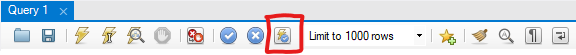
\includegraphics[width=0.8\textwidth]{figs/autoejecucion.png}
    \caption{Botón a desactivar de \texttt{autocommit}.}\label{fig:autoejecución}
\end{figure}

A partir de ahora, todas las consultas y sentencias que ejecutes desde el Workbench formarán parte de una misma transacción hasta que no hagas la confirmación o reviertas los cambios. En otras palabras, la base de datos mantendrá constantemente una transacción abierta, de forma que cuando hagas COMMIT o ROLLBACK se confirman/revierten los cambios y se vuelve a abrir una transacción.

\subsection*{Simular uso simultáneo de la base de datos por varios usuarios}

Ahora tenemos que simular que otro usuario se conecta a nuestra misma base de datos. Para ello, ve a la pestaña con el icono de la casa para que te aparezcan las conexiones guardadas que hay en el MySQL Workbench, y haz doble clic en la misma conexión que has usado antes para conectarse a la base de datos (ver Figura \ref{fig:mysqlwork}).

\begin{figure}[ht]
    \centering
    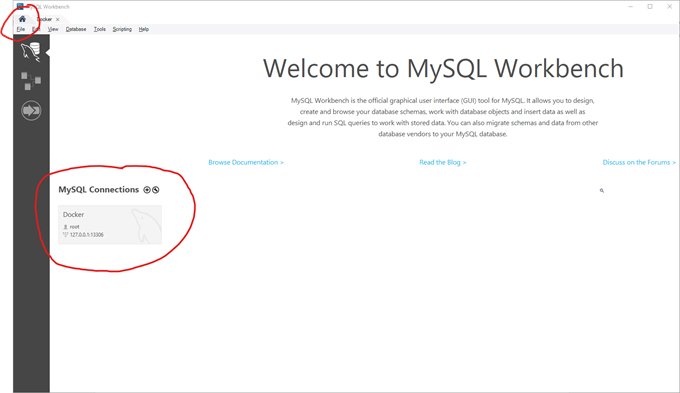
\includegraphics[width=0.9\columnwidth]{figs/mysqlwork.png}
    \caption{Ventana principal de MySQL Workbench.}\label{fig:mysqlwork}
\end{figure}

Podrás comprobar que se te ha abierto una nueva pestaña con una conexión a la base de datos (ver Figura \ref{fig:pestañas}). A todos los efectos, cada pestaña es una conexión independiente, por lo que podemos simular que hay dos usuarios interactuando en la base de datos simultáneamente. Recuerda desactivar el \texttt{autocommit} tanto desde el botón de la pestaña de las consultas como con la sentencia SQL vista en el apartado anterior.

\begin{figure}[ht]
    \centering
    \includegraphics[width=0.6\columnwidth]{figs/pestañasconex.png}
    \caption{Pestañas de conexión.}\label{fig:pestañas}
\end{figure}

\subsection*{Cambios sin confirmar en la base de datos}

En una de las dos pestañas vamos a iniciar una transacción para añadir una nueva película y un nuevo actor a la base de datos. Ejecuta las siguientes sentencias para inicializar una transacción e insertar una fila en la tabla \texttt{film}:

\begin{lstlisting}[language=SQL]
START TRANSACTION;

INSERT INTO peliculas.film (title, description, release_date, 
  language_id, original_language_id, length_minutes) 
VALUES ('Pulp Fiction', 'Pulp Fiction is a 1994 American crime film 
  written and directed by Quentin Tarantino, who conceived it  with 
  Roger Avary.', '1994-05-21', 'es', 'en', 154);
\end{lstlisting}

Comprobamos que en la pestaña en la cual tenemos la transacción abierta la filas aparecen como insertadas (ver Figura \ref{fig:1consulta}):

\begin{lstlisting}[language=SQL]
SELECT * 
FROM film
WHERE title LIKE('Pulp%')
\end{lstlisting}

\begin{figure}[ht]
    \centering
    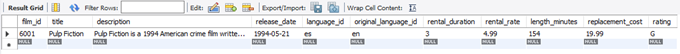
\includegraphics[width=0.9\columnwidth]{figs/1consulta.png}
    \caption{Resultado de la ejecución de la primera consulta.}\label{fig:1consulta}
\end{figure}

Sin embargo, si cambiamos de pestaña para comprobar el otro usuario, al ejecutar la misma consulta podemos observar que la película no aparece (ver Figura \ref{fig:2consulta}):

\begin{lstlisting}[language=SQL]
START TRANSACTION;

SELECT * 
FROM film
WHERE title LIKE('Pulp%');

COMMIT;
\end{lstlisting}

\begin{figure}[ht]
    \centering
    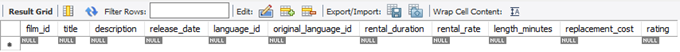
\includegraphics[width=0.9\columnwidth]{figs/2consulta.png}
    \caption{Resultado de la ejecución de la segunda consulta.}\label{fig:2consulta}
\end{figure}

Este es el comportamiento que se podría esperar, puesto que el usuario que ha realizado las inserciones todavía no ha confirmado los cambios y, por tanto, la fila no se ha insertado todavía en la tabla.

Volvemos a la pestaña del usuario que mantiene la transacción abierta y confirmaremos los cambios con la sentencia:

\begin{lstlisting}[language=SQL]
COMMIT;
\end{lstlisting}

La transacción se ha cerrado y los cambios realizados en ella se han convertido en permanentes, por lo que la fila se ha insertado en la tabla de la base de datos y ya es visible para el resto de usuarios. Vamos a comprobarlo cambiando a la otra pestaña y volviendo a ejecutar la consulta:

\begin{lstlisting}[language=SQL]
START TRANSACTION;

SELECT * 
FROM film
WHERE title LIKE('Pulp%');

COMMIT;
\end{lstlisting}

Ahora, tal como muestra la Figura \ref{fig:3consulta} ya aparece la película que insertó el otro usuario, puesto que los cambios han sido confirmados.

\begin{figure}[ht]
    \centering
    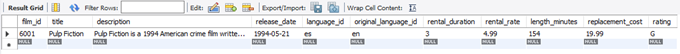
\includegraphics[width=0.9\columnwidth]{figs/3consulta.png}
    \caption{Resultado de la ejecución de la tercera consulta.}\label{fig:3consulta}
\end{figure}

\subsection*{Deshaciendo los cambios con Rollback}

Vamos a comprobar el funcionamiento de la instrucción \texttt{ROLLBACK}. Para ello, en alguna de las dos pestañas de conexión vamos a inicializar una nueva transacción y a eliminar la película que acabamos de añadir. \textbf{Para ello será necesario saber qué ID se le ha asignado a esa película en la base de datos}:

\begin{lstlisting}[language=SQL]
START TRANSACTION;

DELETE FROM film 
WHERE film_id = 6001;
\end{lstlisting}

Los cambios todavía no se han confirmado, por lo que la película debería seguir apareciendo en las otras conexiones que tengamos abiertas. Si consultamos en la pestaña en la que tenemos la transacción abierta, podemos observar que la película se ha eliminado (ver Figura \ref{fig:4consulta}):

\begin{lstlisting}[language=SQL]
SELECT * 
FROM film
WHERE title LIKE('Pulp%');
\end{lstlisting}

\begin{figure}[ht]
    \centering
    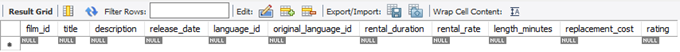
\includegraphics[width=0.9\columnwidth]{figs/4consulta.png}
    \caption{Resultado de la ejecución de la cuarta consulta.}\label{fig:4consulta}
\end{figure}

Supongamos que la eliminación no tendría que realizarse. Gracias a que dicha eliminación está en una transacción todavía abierta, podemos descartar las modificaciones haciendo \texttt{ROLLBACK}:

\begin{lstlisting}[language=SQL]
ROLLBACK;
\end{lstlisting}

Por lo que los cambios quedan descartados y la fila permanece en la tabla correspondiente (ver Figura \ref{fig:5consulta}):

\begin{lstlisting}[language=SQL]
START TRANSACTION;

SELECT * 
FROM film
WHERE title LIKE('Pulp%');

COMMIT;
\end{lstlisting}

\begin{figure}[ht]
    \centering
    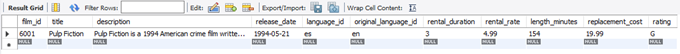
\includegraphics[width=0.9\columnwidth]{figs/5consulta.png}
    \caption{Resultado de la ejecución de la quinta consulta.}\label{fig:5consulta}
\end{figure}

Para obtener información adicional sobre las transacciones en MySQL se puede consultar la documentación oficial en el siguiente enlace:

\url{https://dev.mysql.com/doc/refman/8.0/en/commit.html}

\end{document}
